\documentclass[12pt, a4paper]{article}
\usepackage{fontspec}
\setmainfont{Times New Roman}
\usepackage[UTF8]{ctex}
\usepackage{listings}
\usepackage{array}
\usepackage{geometry}
\geometry{a4paper, scale=0.75}
\usepackage{ctex}
\usepackage{amsmath}
\usepackage{epsfig}
\usepackage{graphicx}
\usepackage{epstopdf}
\usepackage{cite}
\usepackage{indentfirst}
\setlength{\parindent}{2em}
\setlength\parskip{.3 \baselineskip}
\usepackage{graphicx}
\usepackage{float}
\usepackage{subfigure}

\begin{document}
	\begin{center}
		\vspace{0.2in}
		\noindent{\fontsize{20pt}{1em}\selectfont\textbf{通信电路\quad 第六周作业}} \\ [12pt]
		\noindent{\fontsize{20pt}{1em}\textbf{Cadence报告}}  \\ [12pt]
		{\fontsize{14pt}{1.2em}\selectfont
			刘开济\\ [10pt]
			2019010973 \\ [10pt]
		}
	\end{center}
    \section{Clapp Oscillator}
    振荡器设计如下
        \begin{figure}[H]
    	\centering
    	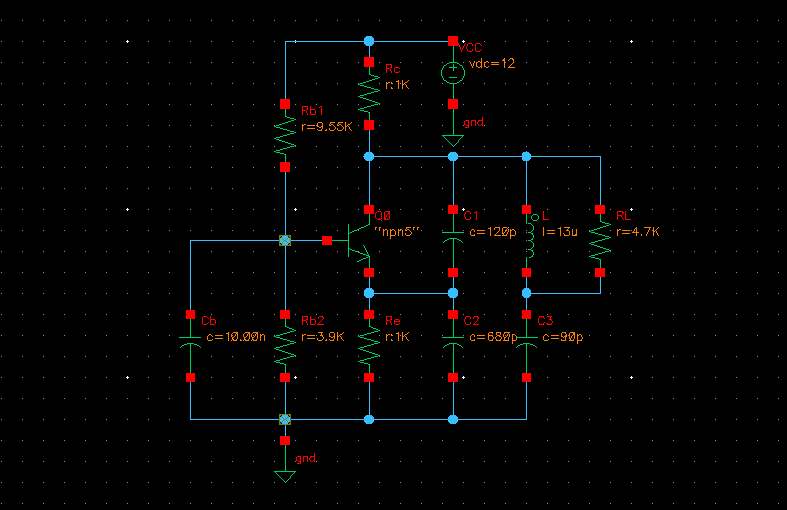
\includegraphics[width = 0.8\textwidth]{clapper-circ}
    	\caption{克拉泼振荡器}
    \end{figure}\par
    振荡器输出如下:
     \begin{figure}[H]
    	\centering
    	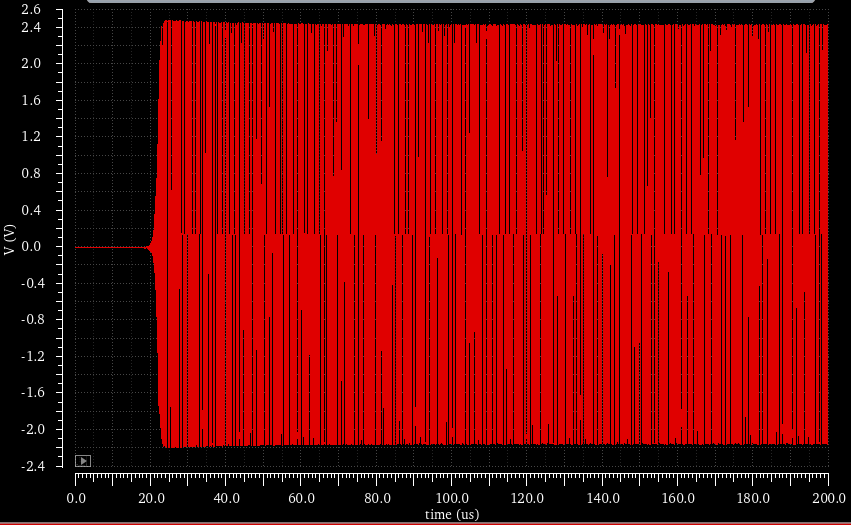
\includegraphics[width = 0.8\textwidth]{clapper-osc}
    	\caption{振荡器输出信号}
    \end{figure}\par
    \section{串联晶体振荡器}
    振荡器电路设计如下:
    \begin{figure}[H]
    	\centering
    	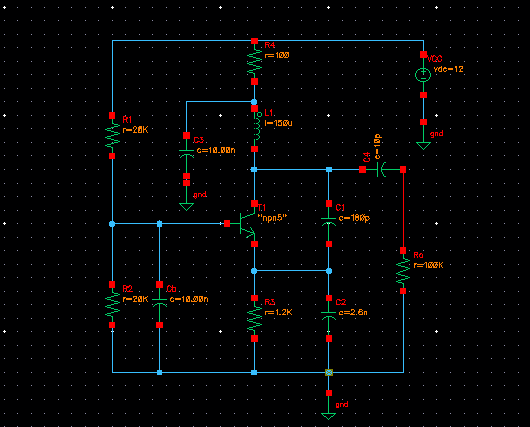
\includegraphics[width = 0.8\textwidth]{crys-circ}
    	\caption{克拉泼振荡器}
    \end{figure}\par
    考察$R_L = 100k\Omega, 33k\Omega, 10k\Omega$的输出波形 :
     \begin{figure}[H]
    	\centering
    	\subfigure[$R_L = 100k \Omega$]{
    		\begin{minipage}[t]{0.48\linewidth}
    			\centering
    			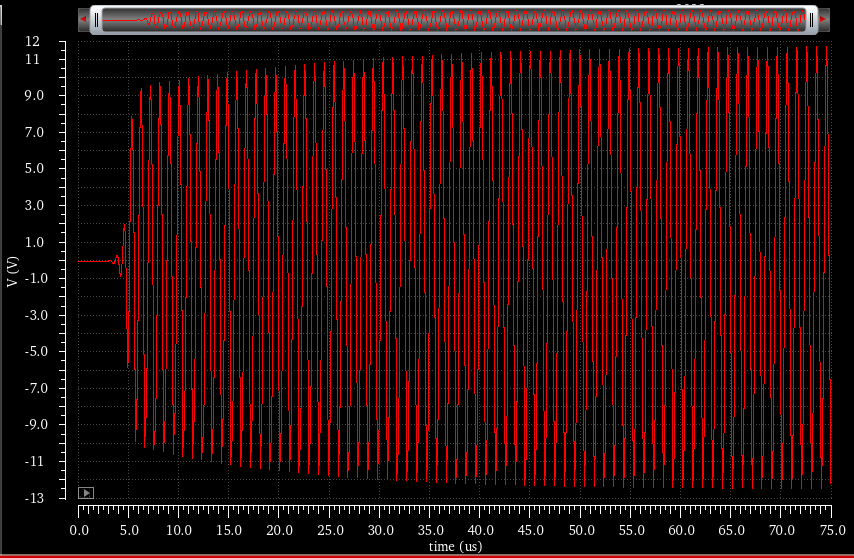
\includegraphics[width=6cm]{crys-RL100}
    			% \caption{传输线LPF\ 50MHz-200MHz幅频特性}
    			%\caption{fig1}
    		\end{minipage}%
    	}
    	\subfigure[$R_L = 33k \Omega$]{
    		\begin{minipage}[t]{0.48\linewidth}
    			\centering
    			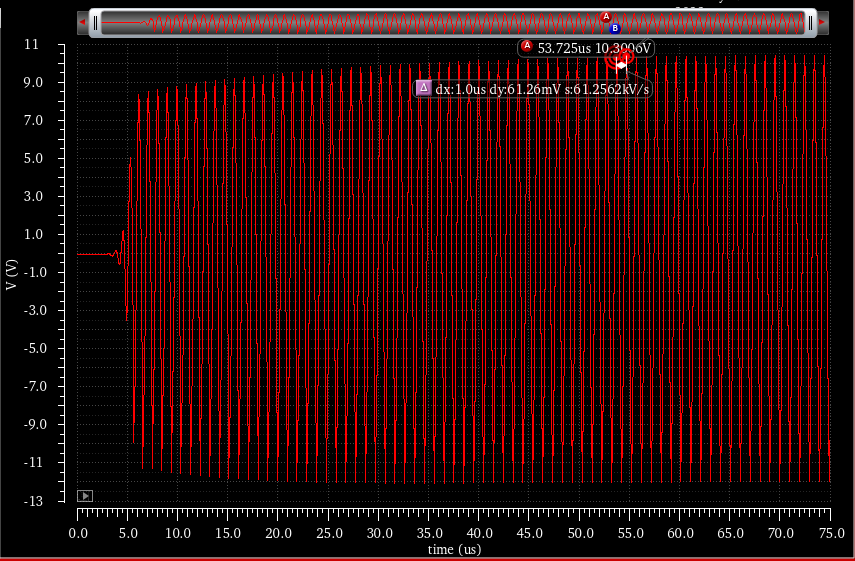
\includegraphics[width=6cm]{crys-RL33}
    			% \caption{传输线LPF\ 50MHz-500MHz幅频特性}
    			%\caption{fig2}
    		\end{minipage}%
    	}%
    	%这个回车键很重要 \quad也可以 
    	
    	\par
    	\subfigure[$R_L = 10k\Omega$]{
    		\begin{minipage}[t]{0.48\linewidth}
    			\centering
    			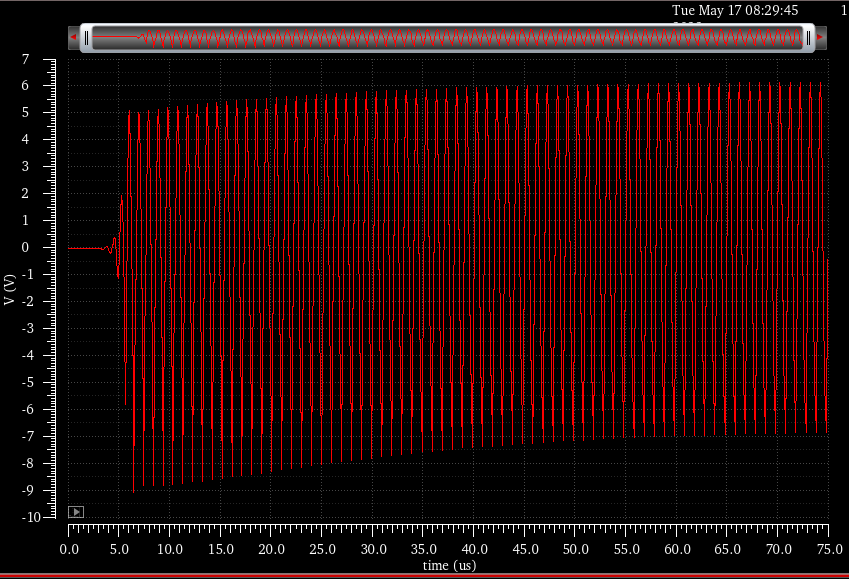
\includegraphics[width=6cm]{crys-RL10}
    			% \caption{传输线HPF\ 50MHz-200MHz幅频特性}
    			%\caption{fig2}
    		\end{minipage}
    	}%
    	\centering
    	\caption{改变$R_L$后输出}
    \end{figure}\par
        通过扫描,得到不同$I_{CQ}$对应的$R_{b2}$数值:
         \begin{center}
        	\tabcolsep8pt
        	\arrayrulewidth2pt
        	\begin{tabular}{| c | c | }
        		\hline
        		$I_{CQ}(mA)$& $R_{b2}(k\Omega)$   \\
        		\hline
        		3.0 & 45.080  \\
        		\hline
        		1.0 & 5.078  \\
        		\hline
        		0.5 & 2.967 \\
        		\hline
        	\end{tabular}
        \end{center} \par
        考察$I_{CQ} = 3mA, 1mA, 0.5mA$的输出波形($R_L = 100k\Omega$) :
    \begin{figure}[H]
    	\centering
    	\subfigure[$I_{CQ} = 3mA$]{
    		\begin{minipage}[t]{0.48\linewidth}
    			\centering
    			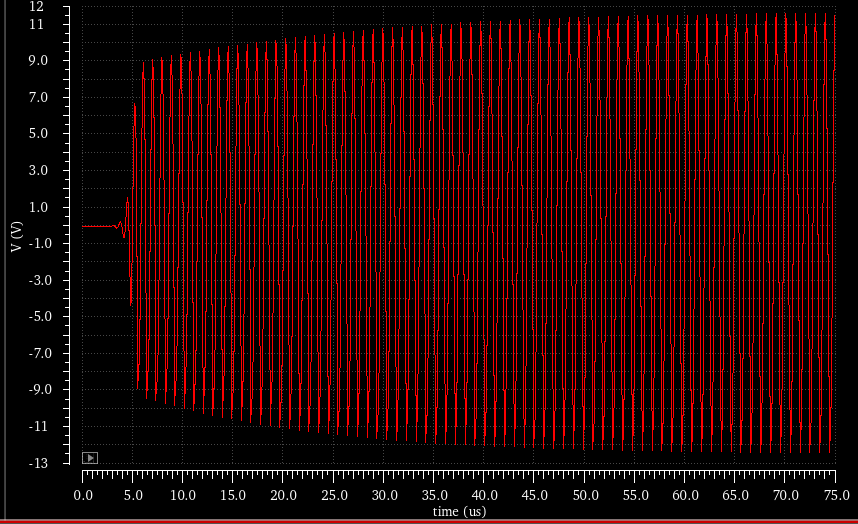
\includegraphics[width=6cm]{crys-ICQ3}
    			% \caption{传输线LPF\ 50MHz-200MHz幅频特性}
    			%\caption{fig1}
    		\end{minipage}%
    	}
    	\subfigure[$I_{CQ} = 1mA$]{
    		\begin{minipage}[t]{0.48\linewidth}
    			\centering
    			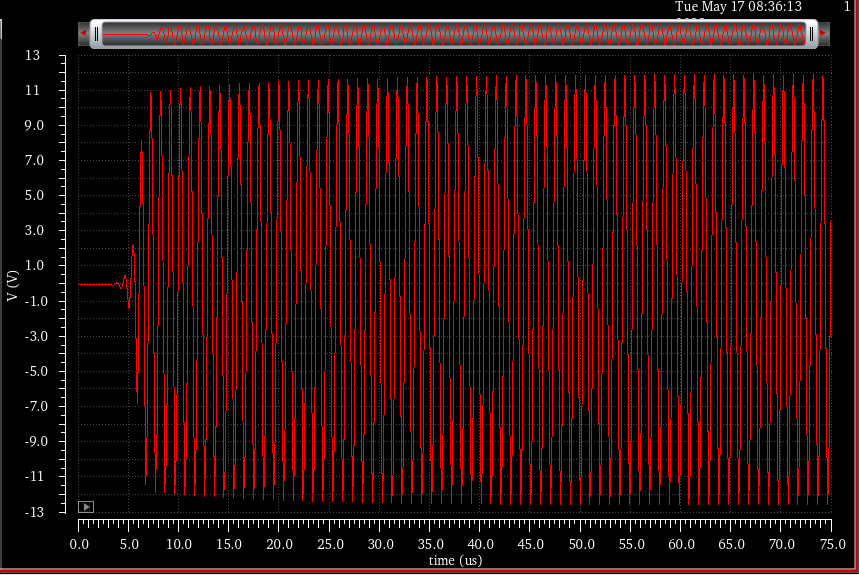
\includegraphics[width=6cm]{crys-ICQ1}
    			% \caption{传输线LPF\ 50MHz-500MHz幅频特性}
    			%\caption{fig2}
    		\end{minipage}%
    	}%
    	%这个回车键很重要 \quad也可以 
    	
    	\par
    	\subfigure[$I_{CQ} = 0.5mA$]{
    		\begin{minipage}[t]{0.48\linewidth}
    			\centering
    			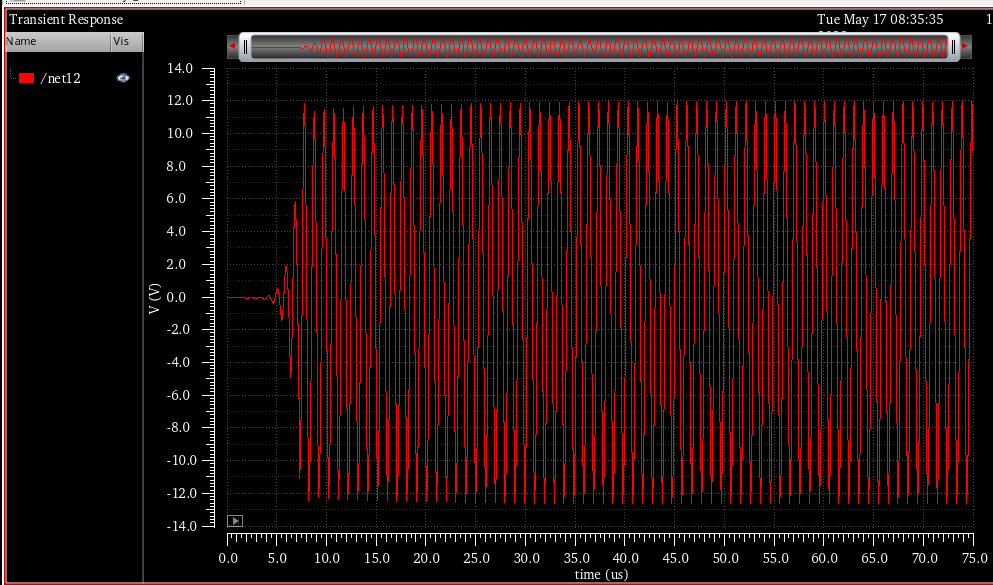
\includegraphics[width=6cm]{crys-ICQ0.5}
    			% \caption{传输线HPF\ 50MHz-200MHz幅频特性}
    			%\caption{fig2}
    		\end{minipage}
    	}%
        	\subfigure[$I_{CQ} = 1mA$]{
    	\begin{minipage}[t]{0.48\linewidth}
    		\centering
    		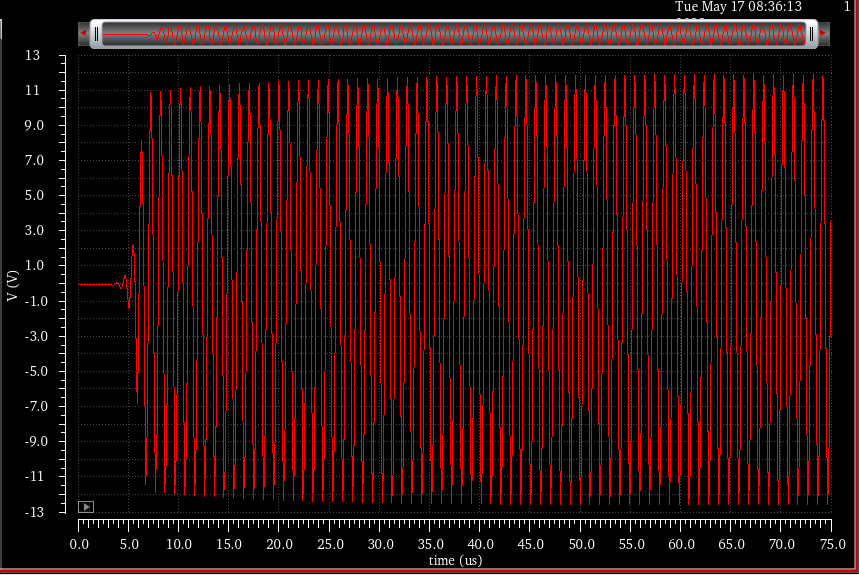
\includegraphics[width=6cm]{crys-ICQ1}
    		% \caption{传输线LPF\ 50MHz-500MHz幅频特性}
    		%\caption{fig2}
    	\end{minipage}%
        }%
    	\centering
    	\caption{改变$I_{CQ}$后输出}
    \end{figure}\par
\end{document}